\documentclass[tikz,border=10pt]{standalone}
\usepackage{tikz}
\usepackage{tikz-cd}
\usetikzlibrary{arrows,automata,shapes,positioning,decorations.pathmorphing}
% \tikzset{->,>=stealth',auto}
\tikzset{->,auto}
\tikzset{>={Latex[width=2mm,length=2mm]}}
\tikzset{state/.style={shape=circle, draw, fill=white, initial text=,
    inner sep=.5mm, minimum size=2mm}}
\tikzset{state with output/.style={shape=rectangle split, rectangle
    split parts=2, draw, fill=white,
    initial text=, inner sep=1mm}}
\tikzset{every node={font=\footnotesize}}
\begin{document}
  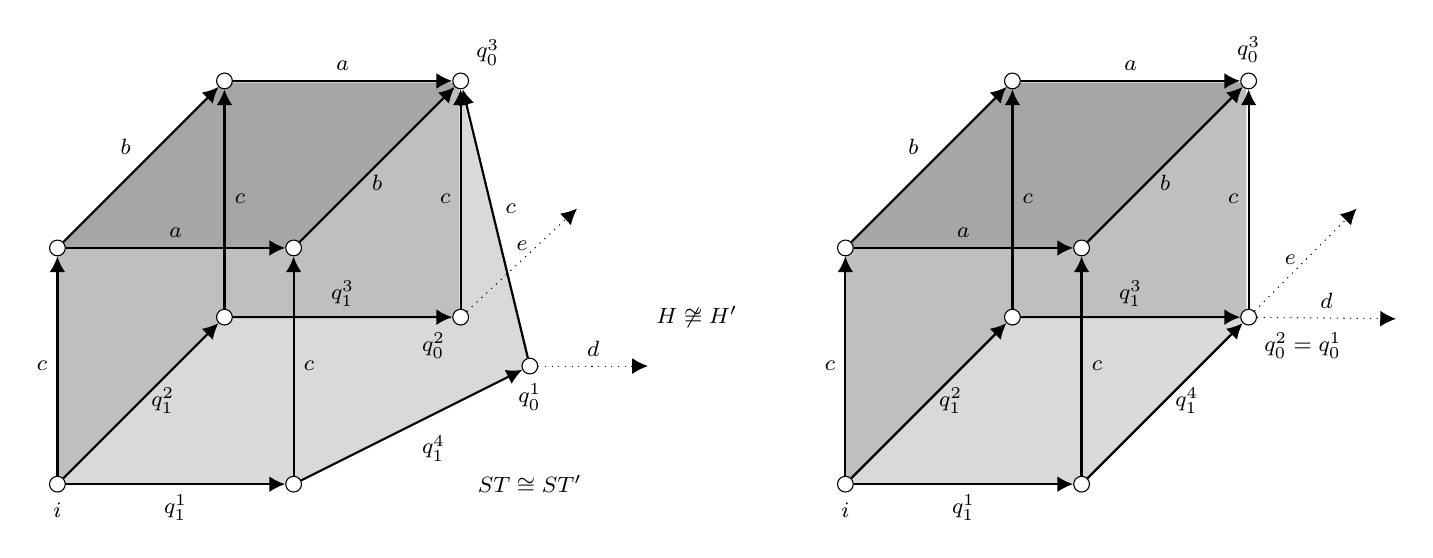
\begin{tikzpicture}[node distance=3cm, align=center]
  \tikzstyle{every node}=[font=\footnotesize]
    \tikzstyle{every state}=[fill=white,shape=circle,inner sep=.5mm,minimum size=3mm]
    \title{Non-isomorphic HDAs collapse into isomorphic STs}
    
    %%%% Left fill
    \path[fill=black!15] (0,0) to (0,3) to (2.1,5.1) to (5.1,5.1) to (6,1.5) to (3,0) to (0,0);
    \path[fill=black!25] (0,0) to (0,3) to (2.1,5.1) to (5.1,5.1) to (5.1,2.1) to (2.1,2.1) to (0,0);
    \path[fill=black!35] (0,3) to (2.1,5.1) to (5.1,5.1) to (3,3) to (0,3);
    
    %%%% right fill
    %\path[fill=black!15] (10,0) to (10,3) to (12.1,5.1) to (15.1,5.1) to (15.1,2.1) to (13,0) to (10,0);
    \path[fill=black!25] (10,0) to (10,3) to (12.1,5.1) to (15.1,5.1) to (15.1,2.1) to (12.1,2.1) to (10,0);
    \path[fill=black!35] (10,3) to (12.1,5.1) to (15.1,5.1) to (13,3) to (10,3);
    \path[fill=black!15] (10,0) to (12.1,2.1) to (15.1,2.1) to (13,0) to (10,0);
    %\path[fill=black!25] (10,0) to (12.1,2.1) to (15.1,2.1) to (13,0) to (10,0);
    %\path[fill=black!25] (10,0) to (10,3) to (12.1,5.1) to (15.1,5.1) to (15.1,2.1) to (13,0) to (10,0);
    
    %%%% Left figure
    \node[state](q1) [label=below:{$i$}]           {};
    \node[state](q2) [right of=q1]                                      {};
    \node[state](q3) [above right of=q1]                                {};
    \node[state](q4) [above right of =q2, label=below left:{$q_0^2$}]{};
    \node[state](q5) [above of=q1]                                      {};
    \node[state](q6) [above of=q2]                                      {};
    \node[state](q7) [above of=q3]                                      {};
    \node[state](q8) [above of=q4, label=above right:{$q_0^3$}]     {};
    \node[state](q9) at (6,1.5)[label=below:{$q_0^1$}]                {};
    
    \node(qe) at (6.6,3.5)  {};
    \node(qd) at (7.5,1.5)  {};
    
    %%%% Right figure
    \node[state](q11) [right=9.9cm, label=below:{$i$}]  {};
    \node[state](q22) [right of=q11]                                        {};
    \node[state](q33) [above right of=q11]                                  {};
    \node[state](q44) [above right of =q22, label=below right:{$q_0^2 = q_0^1$}]  {};
    \node[state](q55) [above of=q11]                                        {};
    \node[state](q66) [above of=q22]                                        {};
    \node[state](q77) [above of=q33]                                        {};
    \node[state](q88) [above of=q44, label=above:{$q_0^3$}]             {};
    
    \node(qee) at (16.5,3.5){};
    \node(qdd) at (17,2.1){};
    
    %%%% HDA isomorphism
    \node(HDA) [right of=q4] {$H \not\cong H'$};
    
    %%%% ST-structure isomorphism
    \node(ST) [right of=q2] {$ST \cong ST'$};
    
    %%%% Special edges
    \draw [->][draw=black, dotted] (q4) to node [above] {$e$} (qe.center);
    \draw [->][draw=black, dotted] (q9) to node [above] {$d$} (qd.center);
    \draw [->][draw=black, dotted] (q44) to node [left] {$e$} (qee.center);
    \draw [->][draw=black, dotted] (q44) to node [above] {$d$} (qdd.center);
    
    %%%% Left figure
    \draw [->][draw=black, thick] (q1) to node [right] {$q_1^2$} (q3);
    \draw [->][draw=black, thick] (q1) to node [below] {$q_1^1$} (q2);
    \draw [->][draw=black, thick] (q3) to node [above] {$q_1^3$} (q4);
    \draw [->][draw=black, thick] (q2) to node [below right] {$q_1^4$} (q9);
    \draw [->][draw=black, thick] (q9) to node [above right] {$c$} (q8);
    
    \draw [->][draw=black, thick] (q1) to node [left] {$c$} (q5);
    \draw [->][draw=black, thick] (q2) to node [right] {$c$} (q6);
    \draw [->][draw=black, thick] (q3) to node [right] {$c$} (q7);
    \draw [->][draw=black, thick] (q4) to node [left] {$c$} (q8);
    
    \draw [->][draw=black, thick] (q5) to node [above left] {$b$} (q7);
    \draw [->][draw=black, thick] (q7) to node [above] {$a$} (q8);
    \draw [->][draw=black, thick] (q5) to node [above] {$a$} (q6);
    \draw [->][draw=black, thick] (q6) to node [below] {$b$} (q8);
    
    %%%% Right figure
    
    \draw [->][draw=black, thick] (q11) to node [right] {$q_1^2$} (q33);
    \draw [->][draw=black, thick] (q11) to node [below] {$q_1^1$} (q22);
    \draw [->][draw=black, thick] (q33) to node [above] {$q_1^3$} (q44);
    \draw [->][draw=black, thick] (q22) to node [right] {$q_1^4$} (q44);
    
    \draw [->][draw=black, thick] (q11) to node [left] {$c$} (q55);
    \draw [->][draw=black, thick] (q22) to node [right] {$c$} (q66);
    \draw [->][draw=black, thick] (q33) to node [right] {$c$} (q77);
    \draw [->][draw=black, thick] (q44) to node [left] {$c$} (q88);
    
    \draw [->][draw=black, thick] (q55) to node [above left] {$b$} (q77);
    \draw [->][draw=black, thick] (q77) to node [above] {$a$} (q88);
    \draw [->][draw=black, thick] (q55) to node [above] {$a$} (q66);
    \draw [->][draw=black, thick] (q66) to node [below] {$b$} (q88);
    
  \end{tikzpicture}
\end{document}